%----------------------------------------------------------------------------------------
%	METODE
%----------------------------------------------------------------------------------------
\section*{METODE PENELITIAN}

Metode yang digunakan dalam penelitian ini ada 6 tahap,  seperti pada Gambar 1. Tahap pertama adalah pengumpulan data Twitter yang diperoleh dari tags.hawksey.info. Langkah selanjutnya adalah melakukan \textit{indexing} yang terdiri dari tokenisasi, normalisasi kata, pembuangan \textit{stopwords}, dan \textit{stemming}. Setelah proses \textit{indexing} dilakukan, tahap selanjutnya adalah melakukan pembagian data menjadi data latih dan data uji. Pada data latih dilakukan pemilihan fitur dengan menggunakan \textit{Mutual Information} (MI). langkah selanjutnya adalah klasifikasi dengan menggunakan \textit{Multinomial Naïve Bayes}. Tahap terakhir adalah evaluasi hasil klasifikasi. 

\begin{figure}[h!] % Gunakan \begin{figure*} untuk memasukkan Gambar
\centering
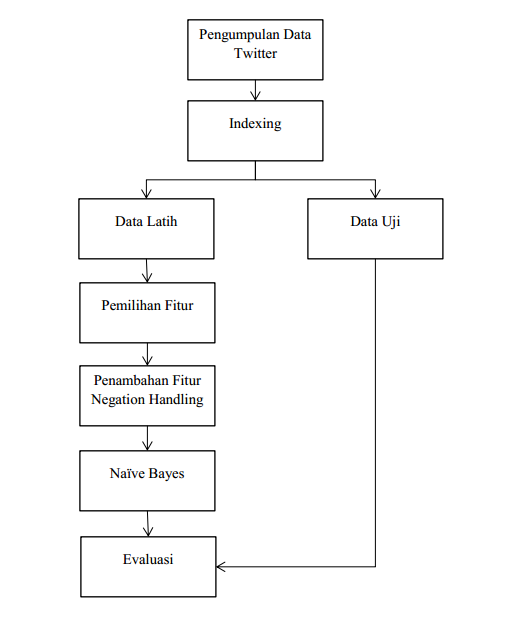
\includegraphics[width=200pt]{langkahkerja.png}
\caption{Metode Penelitian Sentimen Analis Data Twitter Bahasa Indonesia}
\label{fig:tahapan}
\end{figure}

\subsection*{Pengumpulan Data}

Tahapan pertama dalam  penelitian  ini adalah pengumpulan data. Penelitian ini menggunakan data Twitter bahasa Indonesia. Data yang akan diambil dari Twitter adalah data dengan \textit{term} “Kementrian” dan “Pendidikan”. Pada tahap akuisisi data \textit{tweet}, data diperoleh dari tags.hawksey.info. Data yang didapatkan berupa data Excel dengan atribut seperti pada Tabel 1.

\begin{table}[hbt]
	\caption{Struktur Data Response Twitter}
	\centering
	\begin{tabular}{llr}
		
		\cmidrule(r){1-2}
		Atribut & Keterangan \\
		\midrule
		id\_str & id dari \textit{post} twitter \\
		from\_user & \textit{username} pemakai twitter \\
		text & \textit{post} twitter \\
		created\_at & tanggal dan waktu \textit{post} dibuat \\
		geo\_coordinates & koordinat tempat \textit{user} \\
		source & tautan profil \textit{user} \\
		profile\_image\_url & gambar profil dari \textit{user} \\
		user\_followers\_count & jumlah \textit{follower user} \\
		user\_friends\_count & jumlah teman \textit{user} \\
		user\_location & lokasi dari \textit{user} \\
		status\_url & link dari \textit{post} twitter \\
		
		\bottomrule
	\end{tabular}
	\label{tab:strukturdatatwitter}
\end{table}

Dari struktur data yang didapatkan dari sistem tersebut, akan diambil atribut \textit{text} sebagai data untuk diolah sentimennya. Data yang diperoleh dari sistem masih berupa data mentah post user yang belum ada sentimennya. Untuk memberikan sentimen pada data tersebut yang akan digunakan sebagai data latih dilakukan dengan memberikan opini secara manual dengan orang nyata. Jumlah data yang digunakan pada penelitian ini sebanyak 6000 data yang sudah diberi sentimen. 

\subsection*{Indexing}

\textit{Indexing} merupakan sebuah proses untuk melakukan pengindeksan terhadap kumpulan dokumen yang akan disediakan sebagai informasi kepada pemakai. Proses pengindeksan bisa secara  manual ataupun secara otomatis. Dewasa ini, sistem pengindeksan secara manual mulai digantikan oleh sistem pengindeksan otomatis. Adapun tahapan dari pengindeksan adalah tokenisasi, normalisasi kata, pembuangan \textit{stopwords}, dan \textit{stemming}.

\subsection*{Tokenisasi}
Tokenisasi adalah proses pemotongan teks menjadi bagian-bagian yang disebut token, yaitu sebuah \textit{instance} dari urutan karakter dalam beberapa dokumen tertentu yang dikelompokkan bersama sebagai unit semantik yang berguna untuk diproses (\citeauthor{MANNING2008} (\cite*{MANNING2008}).Token bisa berupa paragraf, kalimat, frasa kata tunggal,  sederhana,  dan konsep. Teknik yang digunakan dalam proses tokenisasi adalah segmentasi dan memilah.

Pada penelitian ini token yang dihasilkan berupa kata tunggal yang nantinya akan menjadi term yang akan digunakan sebagai penciri untuk klasifikasi sentiment pada Twitter. Dalam tahap ini dokumen atau data post Twitter diubah menjadi kumpulan term dengan cara menghilangkan mention, URL, tanda baca dan angka pada tweet. Semua huruf pada tweet diubah menjadi huruf kecil. Contoh dari tokenisasi adalah seperti Tabel \ref{tab:tokenizing}.

\begin{table}[hbt]
	\caption{Tokenizing}
	\centering
	\begin{tabular}{llr}
		\toprule
		Input & \multicolumn{2}{c}{Analisis Sentimen} \\
		\midrule
		Output & Analisis & Sentimen \\
		\bottomrule
	\end{tabular}
	\label{tab:tokenizing}
\end{table}

Pada penelitian ini tokenisasi dilakukan dengan menggunakan kode dari Nette yang terdapat di https://github.com/nette/tokenizer.


\subsection*{Penghapusan Stopwords}

Stopwords adalah sebuah kata-kata dalam bahasa tertentu yang sangat umum dan memiliki nilai informasi nol. Meyer et.al.(2008). Stopwords didefinisikan sebagai term yang tidak berhubungan (\textit{irrelevant}) dengan dokumen meskipun kata tersebut sering muncul di dalam dokumen. Contoh \textit{stopwords} dalam bahasa  Indonesia : yang, juga, dari, dia, kami, kamu, aku, saya, ini, itu, atau, dll.
Penghapusan stopwords dilakukan untuk menghilangkan kata dalam daftar kata buang (\textit{stopwords}). Kata tersebut merupakan kata yang jika dihapus tidak mengubah makna dari tweet. Daftar \textit{stopwords} didapatkan dari penelitian Tala (2003) sebanyak 759 kata.


\subsection*{Normalisasi Kata}

Menurut Aziz (2013) tahap normalisasi kata dilakukan dengan penggantian kata yang tidak baku menjadi baku, karena kata yang sudah baku akan cenderung lebih kecil ambiguitas dalam pelafalannya dibanding dengan kata yang tidak baku. Misalnya, kata dengan dapat ditulis dengan "dg" dan "dgn".  Untuk itu perlu dilakukan normalisasi kata dengan cara mengganti kata yang tidak baku dengan kata yang sesuai konteknya (Sproat et al. 2001). Sebelumnya sudah dibuat terlebih dahulu sebuah kamus yang tidak baku dengan kata bakunya, agar memudahkan dalam fungsi penggantian dan kemudian menggantinya dengan kata baku yang telah ada di dalam kamus tersebut. Dataset kata tidak baku dan kata baku yang digunakan sebanyak 3719 baris data. 

\subsection*{Stemming}

\textit{Stemming} adalah  proses  konversi term ke bentuk  umumnya. Dokumen dapat pula diekspansi dengan mencarikan  sinonim  bagi \textit{term} tertentu di  dalamnya. Sinonim adalah kata-kata yang mempunyai pengertian serupa tetapi berbeda dari sudut pandang morfologis. Seperti \textit{stemming},  operasi ini bertujuan menemukan suatu kelompok kata terkait.
\textit{Stemming} merupakan salah satu cara yang digunakan untuk meningkatkan performa IR dengan cara mentransformasi kata-kata dalam sebuah dokumen teks ke kata dasarnya (Agusta, 2009). Tahap \textit{stemming} bertujuan untuk mengurangi jumlah kata dan mendapatkan kata dasar yang benar-benar sesuai.Tahap ini menggunakan algoritme Nazief dan Adriani (1996) untuk menghapus berbagai variasi \textit{prefix} (awalan) dan suffix (akhiran). Kamus kata dasar sebanyak 28.526 kata.

\subsection*{Pembuatan Document Term Matrix (DTM)}

Menurut Nadilah (2016) tahap pembuatan \textit{term document matrix} (TDM) dilakukan untuk membuat matriks jumlah kemunculan suatu kata pada dokumen. \textit{Document Term Matrix} (DTM) merupakan cara yang paling umum digunakan untuk merepresentasikan text. DTM dapat diekspor dari korpus dan digunakan sebagai mekanisme \textit{bag-of-words}. Pendekatan ini menghasilkan matrik dengan id dokumen sebagai baris dan \textit{term} sebagai kolom. Elemen matrik merupakan frekuensi.
Sebagai contoh ada dua dokumen dengan id 1 dan 2 mempunyai kata yang sama yaitu “Nama saya budi dan nama ayah saya budi” dan “nama teman saya budi”.

Pada penelitian ini kolom matriks menunjukkan kata yang ada pada data tweet, sedangkan baris matriks menunjukkan indeks dari dokumen pada kumpulan korpus. Pada penelitian ini satu tweet menandakan satu dokumen.

\subsection*{Pembagian Data}

Tahap selanjutnya adalah pembagian data. Data yang dihasilkan setelah proses indexing dibagi  menjadi  dua subset data yaitu data latih dan data uji dengan perbandingan 70:30. Sebanyak 70 persen data latih dan 30 persen data uji. Data latih ini akan digunakan dalam tahapan pemilihan fitur sementara data uji digunakan untuk melakukan pengujian terhadap sistem klasifikasi yang telah dibuat dalam penelitian ini.

\subsection*{Pemilihan Fitur}

\citeauthor{NARAYANAN2013} (\cite*{NARAYANAN2013}) menyatakan pemilihan fitur  merupakan proses menghilangkan fitur yang berlebihan tapi tetap mempertahakan fitur yang memiliki kemampuan disambiguitas. Pemilihan  fitur mempunyai dua tujuan utama. Pertama, membuat data latih yang digunakan untuk classifier lebih efisien dengan cara mengurangi ukuran kosakata yang efektif. Kedua, pemilihan fitur biasanya dapat meningkatkan akurasi klasifikasi dengan menghilangkan fitur noise (\citeauthor{NARAYANAN2013} \cite*{NARAYANAN2013}). 
Garnes (2009) menyatakan pemilihan fitur secara umum dibagi menjadi dua metode, yaitu unsupervised feature selection dan supervised feature selection. Unsupervised feature selection adalah sebuah metode pemilihan fitur yang tidak menggunakan informasi kelas dalam data latih ketika memilih fitur untuk classifier. Contoh dari Unsupervised feature selection adalah IDF. Supervised feature selection adalah metode pemilihan  fitur yang menggunakan informasi kelas dalam data latih, sehingga untuk menggunakan pemilihan fitur ini harus tersedia sebuah set pre-classied. Contoh dari supervised feature selection adalah Mutual Information (MI) dan Chi-square.


\subsection*{Inverse document frequency (IDF)}

Banyaknya dokumen d yang mengandung term t tertentu disebut DF. Ukuran kepentingan suatu term dari dokumen yang digunakan sebagai penciri adalah nilai DF yang besar, namun nilai dari DF memiliki rentang nilai yang lebar. Inverse document frequency (IDF) adalah inverse dari nilai DF, sehingga ukuran kepentingan suatu term dari dokumen yang akan digunakan penciri yang memiliki nilai kecil dengan rentang yang tidak begitu jauh. Nilai dari IDF disimbolkan dengan  idft  yang ditulis dengan formula [\ref{eq:persamaanidf}]

\begin{equation}
	idf\textsubscript{t} = log(\frac{N}{df\textsubscript{t}})
		\label{eq:persamaanidf}
\end{equation}

sedangkan N adalah banyaknya dokumen dan df\textsubscript{t} adalah banyaknya dokumen didalam koleksi yang mengandung term tertentu.

\subsection*{Mutual information (MI)}

Salah satu seleksi fitur yang sering digunakan untuk menghitung bobot dari fitur adalah \textit{Mutual information}. MI menunjukan seberapa banyak informasi ada atau tidaknya sebuah term memberikan konstribusi dalam membuat keputusan klasifikasi secara benar atau salah. Nilai dari MI disimbolkan dengan notasi I, dimana [\ref{eq:persamaanmi}]

\begin{equation}
	\begin{split}
		\tiny
		I(U;C) = \sum\limits_{et\in\{1,0\}}\sum\limits_{ec\in\{1.0\}} P(U = et, C = ec) \\
		log_2 \frac{P(U = et,C =ec)}{P(U = et)P(C = ec)} 
		\label{eq:persamaanmi}
		\normalsize
	\end{split}
\end{equation}

sedangkan U adalah variabel acak dengan nilai-nilai et = 1 (dokumen berisi term t) dan et = 0 (dokumen tidak mengandung t), dan C adalah variabel acak dengan nilai-nilai ec = 1 (dokumen di kelas c ) dan ec = 0 (dokumen tidak di kelas c). Nilai dari I juga bisa dijabarkan menjadi seperti persamaan  [\ref{eq:milanjut}]

\begin{equation}
	\begin{split}
		\tiny
		\frac{N11}{N}log_2\frac{NN11}{N1.N.1} + \frac{N01}{N}log_2\frac{NN01}{N0.N.1} + \\
		\frac{N10}{N}log_2\frac{NN11}{N1.N.0} + \frac{N00}{N}log_2\frac{NN00}{N0.N.0}
		\label{eq:milanjut}
		\normalsize
	\end{split}
\end{equation}

dengan N adalah jumlah dokumen yang memiliki nilai-nilai et dan ec yang ditunjukan oleh dua subscript. Sebagai contoh, N10 adalah jumlah dokumen yang mengandung term t (et = 1) dan tidak dalam c (ec = 0). N1. = N10 + N11 adalah jumlah dokumen yang berisi term t (et = 1) dan untuk menghitung dokumen independen keanggotaan kelas (ec = {0, 1}). N adalah jumlah total dokumen atau N= N00 + N01 + N10 + N11.

\subsection*{Chi-Square (X\textsuperscript{2})}
x\textsuperscript{2} biasanya digunakan digunakan dalam menguji independensi dari dua variabel  yang berbeda. Hipotesis nol jika kedua variabel saling bebas satu sama lain jika nilai dari x\textsuperscript{2} tinggi maka hubungan kedua variabel tersebut semakin erat. Dalam seleksi fitur x\textsuperscript{2} digunakan untuk mengukur independensi term t dan kelas c. hipotesis yang diuji adalah term dan kelas benar-benar independen, artinya fitur ini tidak berguna untuk mengelompokkan dokumen. Semakin tinggi nilai maka semakin rendah nilai independensinya. Persamaan dari x\textsuperscript{2}  dapat ditulis sebagai [\ref{eq:chi}]

\begin{equation}
	\begin{split}
		\tiny
		X^2(D, t, c) = \sum\limits_{et\in\{1,0\}}\sum\limits_{et\in\{1,0\}} \frac{(N_{etec} - E_{etec})^2}{E_{etec}}
		\label{eq:chi}
		\normalsize
	\end{split}
\end{equation}

Sedangkan D adalah variabel acak dengan nilai-nilai et = 1 adalah dokumen berisi term t dan et = 0 adalah dokumen yang tidak mengandung t, ec = 1 adalah dokumen di kelas c dan ec = 0 adalah dokumen tidak di kelas c. N adalah frekuensi yang diamati dalam dokumen D dan E adalah frekuensi yang diharapkan. Pengambilan keputusan dilakukan berdasarkan nilai dari masing-masing kata. Kata yang memiliki nilai x2  di atas nilai kritis pada taraf nyata adalah kata yang akan dipilih sebagai penciri dokumen. Kata yang dipilih sebagai penciri merupakan kata yang memiliki pengaruh terhadap kelas c. Nilai kritis  x2  untuk taraf nyata  $ \alpha $ yang digunakan dalam penelitian ini ditunjukkan pada Tabel  \ref{tab:chisquare}.

\begin{table}[hbt]
	\caption{Nilai kritis untuk taraf nyata $ \alpha $}
	\centering
	\begin{tabular}{llr}
		\toprule
		$ \propto $ & Nilai Kritis \\
		\midrule
		0.050 & 3.840 \\
		0.010 & 6.630 \\
		0.005 & 7.880 \\
		\bottomrule
	\end{tabular}
	\label{tab:chisquare}
\end{table}

Pada penelitian ini pemilihan fitur yang digunakan adalah MI dan IDF yang nantinya dapat dilihat perbandingan hasil akurasinya.

\subsection*{Klasifikasi}
Tahapan klasifikasi ini bertujuan mengklasifikasikan atau mengkategorikan data tweet menjadi tiga kelas sentimen yaitu sentimen positif, negatif dan netral.  Fungsi klasifikasi secara umum untuk memetakan suatu dokumen ke dalam kategori tertentu yaitu: [\ref{eq:klasifikasi}]

\begin{equation}
	\begin{split}
		\tiny
		\gamma : X -> C
		\label{eq:klasifikasi}
		\normalsize
	\end{split}
\end{equation}

Secara umum fungsi ini yang akan dipakai untuk mengelompok data ke dalam himpunan kelas atau kategori yang ada, dengan X adalah kumpulan dokumen dan C merupakan kategori. Ada beberapa algoritme yang dapat dilakukan untuk melakukan klasifikasi data yaitu algoritme berbasis peluang dan algoritme berbasis vektor. 

Algoritme berbasis peluang yaitu Bernouli Naïve Bayes dan Multinomial Naïve Bayes.Sedangkan algoritme berbasis vektor yaitu Rocchio dan k nearest neighbor (kNN) (\citeauthor{MANNING2008} \cite*{MANNING2008}). Pada algoritme berbasis peluang, penentuan kelas pada sebuah dokumen atau data adalah dengan cara menghitung peluang keberadaan data tersebut dalam suatu kelas. Sedangkan pada algoritme berbasis vektor, penentuan kelas pada sebuah data dilakukan dengan cara menghitung jarak data tersebut ke centroid suatu kelas.

Algoritme Naïve Bayes dengan model multinomial dan model Bernoulli digunakan karena proses yang sederhana dan mudah diaplikasikan pada berbagai keadaan sehingga tidak akan mengalami kegagalan secara keseluruhan pada hasilnya (\citeauthor{MANNING2008} \cite*{MANNING2008}).Pada model       Naïve Bayes Bernouli dokumen diwakili oleh atribut biner yang menunjukkan bahwa ada dan tidak ada term dalam dokumen. Frekuensi kemunculan term dalam dokumen tidak ikut diperhitungkan. Sedangkan Multinomial Naïve Bayes, dokumen diwakili oleh kemunculan term dari dokumen. Pada model ini, sebelumnya dibuat asumsi jika kemunculan masing-masing term t bersifat independen antara satu term dengan yang lainnya. \citeauthor{MANNING2008} (\cite*{MANNING2008}) menyatakan dengan menggunakan nilai dari \textit{\^{P}}$(c|d) $ peluang suatu dokumen d di dalam kelas c dapat ditulis seperti persamaan [\ref{eq:klasifikasi1}] 

\begin{equation}
	\begin{split}
		\tiny
		\hat{P}(c|d) \propto P(c) \prod_{1\leq k \leq nd}P(t_k|c)
		\label{eq:klasifikasi1}
		\normalsize
	\end{split}
\end{equation}

dengan  \textit{\^{P}}$(t_{k}|c) $ adalah peluang dari suatu term $ t_{k} $ muncul pada dokumen yang dikeutahui memiliki kelas c. Pendugaan parameter  \textit{\^{P}}$(t_{k}|c) $ dihitung dengan cara seperti persamaan [\ref{eq:klasifikasi2}]

\begin{equation}
	\begin{split}
		\tiny
		\hat{P}(t_k|C) = \frac{T_{ct}}{\sum _{t' \in V} T_{ct'}}
		\label{eq:klasifikasi2}
		\normalsize
	\end{split}
\end{equation}

dengan $ T_{ct} $ adalah jumlah kemunculan term t dalam dokumen training yang berada di kelas c.  adalah jumlah seluruh term yang muncul berulang kali pada dokumen yang sama.

\citeauthor{MANNING2008} (\cite*{MANNING2008}) menyatakan Term tidak selalu muncul pada salah satu kelas saat dilakukan klasifikasi sehinggga nilai \textit{\^{P}}$(t_{k}|c) $   yang dihasilkan adalah nol. Untuk mengatasi permasalahan tersebut, digunakan laplace smoothing, yaitu menambahkan frekuensi term sebanyak 1. sehingga perhitungan dari  \textit{\^{P}}$(t_{k}|c) $  menjadi seperti persamaan [\ref{eq:klasifikasi3}] 

\begin{equation}
	\begin{split}
		\tiny
		\hat{P}(t|c) = \frac{T_{ct} + 1}{\sum _{t' \in V} T_{ct'} + B}
		\label{eq:klasifikasi3}
		\normalsize
	\end{split}
\end{equation}

Algoritme Rocchio merepresentasikan data ke dalam sebuah vector dengan  menggunakan perhitungan jarak atau kemiripan suatu data dengan pusat sebuah kelas. Algoritme Rocchio membagi ruang vektor menjadi beberapa bagian berdasarkan centroid yang ada. Nilai centroid merupakan hasil perhitungan rata- rata jarak pada setiap data atau dokumen. Nilai centroid dapat dihitung dari persamaan [\ref{eq:klasifikasi4}] 

\begin{equation}
	\begin{split}
		\tiny
		|\vec{x}-\vec{y}| = \sqrt{\sum^{m}_{i=1}(x_{i}-y_{i})^2} 
		\label{eq:klasifikasi4}
		\normalsize
	\end{split}
\end{equation}

dimana $ |\vec{x}-\vec{y}| $  merupakan jarak data uji x ke kelas y, $ x_{i} $ merupakan data uji ke-i, $ y_{i} $ merupakan kelas ke-i, dan m adalah banyak data. Sedangkan untuk menghitung kemiripan antara dua vektor dokumen, didefinisikan seperti persamaan [\ref{eq:klasifikasi5}] 

\begin{equation}
	\begin{split}
	\tiny
	sim(d_{1},d_{2}) = \frac{\vec{V}(d_{1})\vec{V}(d_{2})}{|\vec{V}(d_{1})||\vec{V}(d_{2}|} 
	\label{eq:klasifikasi5}
	\normalsize
	\end{split}
\end{equation}

dimana $ sim(d_{1},d_{2}) $ merupakan kemiripan dokumen $ d_{1} $ dan dokumen $ d_{2} $ , $ \vec{V}(d_{1}) $ merupakan panjang vektor dokumen $ d_{1} $ , dan$  \vec{V}(d_{2}) $ merupakan panjang vektor dokumen$ d_{2} $. 

Menurut \citeauthor{ALKHATIB2013} (\cite*{ALKHATIB2013}) kNN merupakan algoritme klasifikasi berbasis vector yang sederhana. Algoritme kNN mendefinisikan vektor dokumen yang berdekatan memiliki kelas yang sama. Algoritme ini menggunakan ukuran kemiripan suatu data dengan membandingkan data uji dengan data latih. Perhitungan jarak data uji dengan data latih dapat dihitung dengan menggunakan persamaan Euclidean sebagai berikut

\begin{equation}
	\begin{split}
		\tiny
		|d(x,y)| = \sqrt{\sum^{m}_{i=1}(x_{i}-y_{i})^2} 
		\label{eq:klasifikasi6}
		\normalsize
	\end{split}
\end{equation}

dimana d(x,y)  merupakan jarak data uji x ke data latih y, $ x_{i} $ merupakan data uji ke-i, $ y_{i} $ merupakan data latih ke-i, dan m adalah banyak data. 

Penelitian ini menggunakan algoritme Multinomial Naïve Bayes dalam mengklasifikasikan data tweet. Penggunaan model klasifikasi ini dikarenakan proses yang sederhana dan mudah diaplikasikan pada berbagai keadaan sehingga tidak akan mengalami kegagalan secara keseluruhan pada hasilnya (\citeauthor{MANNING2008} \cite*{MANNING2008}).  


\subsection*{Evaluasi}
Langkah selanjutnya adalah melakukan evaluasi. Evaluasi bertujuan untuk mengetahui tingkat akurasi hasil klasifikasi data menggunakan metode Multinomial Naïve Bayes terhadap data uji. Tahap evaluasi dilakukan untuk mengetahui tingkat akurasi dari hasil penggunaan indexing, pemilihan fitur, serta klasifikasi pada data uji. Pengujian penelitian ini dilakukan pada data uji terhadap fungsi klasifikasi yang sudah di training. Token dari hasil seleksi fitur, akan dihitung peluangnya berdasarkan kelas-kelasnya dari dokumen Twitter. Setelah itu, membandingkannya dengan kelas aktual dari data uji dan kelas hasil prediksi dengan menggunakan confusion matrix. Isi dari confusion matrix adalah jumlah kasus-kasus yang telah diklasifikasikan dengan benar dan kasus-kasus yang salah diklasifikasikan.Evaluasi digunakan untuk mengukur efektivitas dari sistem IR. Dua pengukuran yang sering digunakan dalam IR adalah precision dan recall.

\subsection*{Precision}
Precision merupakan teknik untuk evaluasi yang didefinisikan sebagai presentase dokumen yang di-retrieve yang benar-benar relevan. [\ref{eq:precision}]

\begin{equation}
	\begin{split}
		\tiny
		Precision = \frac{(relevant items retrieved)}{(retrieved items)} \\ 
		= P(relevant|retrieved)
		\label{eq:precision}
		\normalsize
	\end{split}
\end{equation}

\subsection*{Recall}
Recall adalah teknik evaluasi untuk menemukan semua item yang relevan dari dalam koleksi dokumen dan iddefinisikan sebagai presentase dokumen yang relevan. [\ref{eq:recall}]

\begin{equation}
\begin{split}
\tiny
Recall = \frac{(relevant items retrieved)}{(relevant items)} \\ 
= P(retrieved|relevant)
\label{eq:recall}
\normalsize
\end{split}
\end{equation}

Konsep tersebut dapat diperjelas pada tabel \ref{tab:konsep}.

\begin{table}[hbt]
	\caption{Tabel Kontigensi}
	\centering
		\begin{tabular}{*{3}{c}}%%{llr}
			\toprule
			aasd & Relevant & Not Relevant \\
			\midrule
			Retrieved & True positive (tp) & False positives (fp) \\
			Not Retrieved & False negatives (fn) & True negatives (tn) \\
			\bottomrule
		\end{tabular}

	\label{tab:konsep}
\end{table}

Maka didapatkan rumus seperti berikut [\ref{eq:evaluasi}]

\begin{equation}
\begin{split}
\tiny
P = tp/(tp+fp) \\ 
R = tp/(tp+fn)
\label{eq:evaluasi}
\normalsize
\end{split}
\end{equation}

\subsection*{Accuracy}
Selain Precision dan Recall, keakuratan sentiment analisis juga dinilai dari akurasinya, untuk menghitung akurasi digunakan rumus seperti berikut dan mengacu tabel \ref{tab:konsep} [\ref{eq:akurasi}]

\begin{equation}
\begin{split}
\tiny
accuracy = (tp+tn)/(tp+fp+fn+tn)
\label{eq:akurasi}
\normalsize
\end{split}
\end{equation}

\subsection*{F-measure}
Pengukuran yang lain adalah F-measure yang merupakan \textit{weighted harmonic mean} dari \textit{precision} dan \textit{recall}. [\ref{eq:fmeasure}]

\begin{equation}
\begin{split}
\tiny
F = \frac{1}{\alpha \frac{1}{p} + (1 - \alpha)\frac{1}{R}} \\
= \frac{(\beta^2 + 1)PR}{\beta^2P + R} \\
where \beta^2 = \frac{1 - \alpha}{\alpha}
\label{eq:fmeasure}
\normalsize
\end{split}
\end{equation}

Dimana$  \alpha \in $ [0,1] dan$  \beta^2 \in $ [0, $ \Psi $]

Balanced F-measure menyamakan bobot dari precision dan recall, yang berarti membuat $ \alpha $ = 1/2 atau $ \beta $ = 1. Ketika menggunakan $ \beta $ = 1, formula dapat disederhanakan sebagai berikut  [\ref{eq:fmeasuredua}]

\begin{equation}
	\begin{split}
		\tiny
		F_\beta = \frac{2PR}{P + R}
		\label{eq:fmeasuredua}
		\normalsize
	\end{split}
\end{equation}

dimana P adalah \textit{precision} , dan R adalah \textit{recall}.


\subsection*{Jadwal Kegiatan}
Penelitian ini akan dilakukan selama 4.5 bulan dengan rincian kegiatan seperti tercantum pada Tabel \ref{tab:jadwal}.
\begin{table*}[t!]
	\begin{center}
		\caption{Rencana Jadwal Penelitian}
		\label{tab:jadwal}
		\footnotesize
		\begin{tabular}{|l|c|c|c|c|c|c|c|c|c|c|c|c|c|c|c|c|c|c|}
			\hline
			\multirow{2}{*}{Kegiatan}&\multicolumn{2}{c|}{1}&\multicolumn{4}{c|}{2}&\multicolumn{4}{c|}{3}&\multicolumn{4}{c|}{4}&\multicolumn{4}{c|}{5}\\
			\cline{2-19}
			&3&4&1&2&3&4&1&2&3&4&1&2&3&4&1&2&3&4\\
			\hline
			Penyusunan Proposal Skripsi&\cellcolor{black}&\cellcolor{black}&\cellcolor{black}&\cellcolor{black}&&&&&&&&&&&&&&\\
			\hline
			Kolokium&&&&&\cellcolor{black}&&&&&&&&&&&&&\\
			\hline
			Perbaikan proposal&&&&&&\cellcolor{black}&&&&&&&&&&&&\\
			\hline
			Pengambilan data lapangan&&&&&&\cellcolor{black}&\cellcolor{black}&\cellcolor{black}&&&&&&&&&&\\
			\hline
			Pengolahan dan analisis data&&&&&&&&\cellcolor{black}&\cellcolor{black}&\cellcolor{black}&\cellcolor{black}&&&&&&&\\
			\hline
			Penulisan draft skripsi&&&&&&&&&&&&\cellcolor{black}&\cellcolor{black}&\cellcolor{black}&\cellcolor{black}&&&\\
			\hline
			Uji petik&&&&&&&&&&&&&&&&\cellcolor{black}&&\\
			\hline
			Sidang skripsi&&&&&&&&&&&&&&&&&\cellcolor{black}&\\
			\hline
			Perbaikan laporan penelitian&&&&&&&&&&&&&&&&&&\cellcolor{black}\\
			\hline
		\end{tabular}
		\normalsize
	\end{center}
\end{table*}